\documentclass[12pt,addpoints]{exam}
\usepackage[utf8]{inputenc}
\usepackage[T1]{fontenc}
\usepackage[brazil]{babel}
\usepackage[a4paper, margin=2cm]{geometry}
\usepackage{graphicx, amsmath, amsfonts, amssymb, xcolor, url, tikz, pgfplots, subfigure}

\newcommand{\disciplina}{Laboratório de Princípios de Comunicações}
\newcommand{\periodo}{2023.1}
\newcommand{\avaliacao}{Guia de Experimentos 2}
\newcommand{\tema}{Filtragem de sinais. Relação sinal-ruído.}
%\newcommand{\professor}{Leocarlos B.\ S.\ Lima e Edson P.\ da Silva}
%\newcommand{\professor}{Edmar Candeia Gurjão e Luciana Veloso}
\newcommand{\professor}{Edson P.\ da Silva e Luciana Veloso}
%\newcommand{\professor}{Bruno\ B.\ Albert e Edson P.\ da Silva}
%\newcommand{\professor}{Adolfo Herbster e Bruno Albert}
%\newcommand{\professor}{Edson Porto e Bruno Albert}
% \newcommand{\professor}{Edmar Gurjão e Bruno Albert}
%\newcommand{\professor}{Luciana Veloso e Bruno Albert}

\pagestyle{head}
\firstpageheader{}{}{}
\runningheader{Lab.\ Princ.\ Comunicações}{\avaliacao}{Página \thepage}
\runningheadrule
\pointpoints{ponto}{pontos}
\newcommand{\myscale}{0.4}
\newtheorem{exemplo}{Exemplo}[section]

\begin{document}

\noindent \includegraphics[height=2cm]{../Figuras/UFCGLogo.png} \hfill
\begin{minipage}{.66\textwidth} \large \centering \vspace{-1.8cm}
    Universidade Federal de Campina Grande -- UFCG \\
    Unidade Acadêmica de Engenharia Elétrica -- UAEE \\
    Curso de Graduação em Engenharia Elétrica
\end{minipage}
\hfill \includegraphics[height=2cm]{../Figuras/DEELogo.png} \\[12pt]

\noindent
\begin{tabular*}{\textwidth}{l @{\extracolsep{\fill}} r @{\extracolsep{6pt}} l}
    \textbf{\disciplina} && \\
    Período \periodo && \\
    \textbf{\avaliacao} && \\
    Tema(s): \tema && \\
    Professor(es): \professor && \\
\end{tabular*}
\noindent\rule[2ex]{\textwidth}{2pt}

\section{Introdução}

O presente guia descreve atividades experimentais a serem realizadas na disciplina Laboratório de Princípios de Comunicações do curso de graduação em Engenharia Elétrica da Universidade Federal de Campina Grande -- UFCG.

Os experimentos propostos deverão ser realizados no Laboratório de Princípios de Comunicações -- LPC, localizado na Central de Laboratórios da Unidade Acadêmica de Engenharia Elétrica da UFCG, empregando:
\begin{itemize}
    \item Computador com software GNU Radio Companion -- GRC (\url{http://gnuradio.org/}) instalado;
    \item Módulo USRP (do inglês \textit{Universal Software Radio Peripheral}) para transmissão e recepção de sinais numa abordagem conhecida como Rádio Definido por Software -- RDS.
\end{itemize}

Na seção \ref{sect:Preparacao} deste guia, propõe-se um conjunto de atividades de preparação a serem desenvolvidas pelo aluno antes da aula em que serão realizadas as práticas experimentais. Sem a realização prévia destas atividades pelo aluno, as práticas experimentais propostas ficarão comprometidas, tanto no tempo necessário para sua realização quanto no aproveitamento pelo aluno. Por essa razão, %\textbf{O aluno deverá realizar a Preparação na plataforma Moodle para ter acesso ao Relatório do Experimento}.
\textbf{o aluno só poderá realizar os experimentos em laboratório se apresentar ao professor no início da aula os resultados da preparação proposta}. 

% A aula terá duração de duas horas e o aluno deverá responder as questões do experimento que estão na parte final do guia, na atividade {\it Relatório do Experimento 2} na plataforma Moodle. %
A aula terá duração de duas horas e o aluno deverá entregar ao seu término, por escrito, respostas às questões referentes aos experimentos realizados propostas na Folha de Respostas (parte final do guia).

% Na seção \ref{sect:Preparacao} deste guia, propõe-se um conjunto de atividades de preparação a serem desenvolvidas pelo aluno antes da aula em que serão realizadas as práticas experimentais. Sem a realização prévia destas atividades pelo aluno, as práticas experimentais propostas ficarão comprometidas, tanto no tempo necessário para sua realização quanto no aproveitamento pelo aluno. Por essa razão, \textbf{O aluno deverá realizar a Preparação na plataforma Moodle para ter acesso ao Relatório do Experimento}. % \textbf{o aluno só poderá realizar os experimentos em laboratório se apresentar ao professor no início da aula os resultados da preparação proposta}. 

% A aula terá duração de duas horas e o aluno deverá responder as questões do experimento que estão na parte final do guia, na atividade {\it Relatório do Experimento 2} na plataforma Moodle. % A aula terá duração de duas horas e o aluno deverá entregar ao seu término, por escrito, respostas às questões referentes aos experimentos realizados propostas na Folha de Respostas (parte final do guia).

\section{Objetivos}

As práticas experimentais aqui propostas têm por objetivos:
\begin{itemize}
    \item Simular e analisar a aplicação de filtros a sinais;
    \item Investigar o conceito de relação sinal-ruído.
\end{itemize}

\section{Preparação} \label{sect:Preparacao}

\subsection{Estudo}

Revise e pesquise sobre os conceitos:
\begin{itemize}
    \item Filtros passa-baixas, passa-faixa e passa-altas;
    \item Relação sinal-ruído;
    \item Largura de faixa de sinais em banda básica e passa-faixa; 
    \item Largura de faixa (banda passante) de sistemas, canais ou filtros.
\end{itemize}

\subsubsection{Filtros digitais}
\label{sec:filtros}

Um sinal discreto no tempo, como um sinal contínuo no tempo, pode ser representado por uma função da frequência chamada de \textit{espectro de frequências} do sinal.  

Filtragem é um processo pelo qual o espectro de frequências de um sinal pode ser modificado de acordo com alguma especificação desejada. A filtragem pode ser usada para atenuar um ruído que está contaminando um sinal, para reduzir distorções, separar dois ou mais sinais que estejam compartilhando um meio de comunicação, analisar as componentes de frequência de um sinal, desmodular sinais, recuperar um sinal contínuo a partir de sua versão amostrada no tempo e limitar em faixa de frequências os sinais.

Um filtro digital é um sistema digital que pode ser usado para filtrar sinais discretos no tempo. Ele pode ser implementado por software, por hardware ou por uma combinação dos dois.

\subsubsection{Projeto de Filtros Digitais FIR } \label{sec:fir}

Um projeto de filtros digitais envolve três passos básicos:
\begin{enumerate}
    \item especificação das propriedades desejadas do sistema;
    \item aproximação dessas especificações utilizando um sistema causal
    discreto no tempo; e
    \item realização do sistema utilizando aritmética de precisão finita.
\end{enumerate}

\begin{table}[b]
\begin{center}
\begin{tabular}{lll}  \\ \hline
Tipo de filtro & Magnitude $\left|H_d(\Omega)\right|$ & Resposta ao impulso $h_d(n)$  \\ \hline
&  & \\
Passa Baixa &  $|H_d(\Omega)|= \begin{cases}
1,  \left|\Omega\right| < \Omega_c \\
0 , \Omega_c < \left|\Omega\right| \leq \pi 
\end{cases}$
& 
$h_d(n)=\begin{cases}
\frac{\Omega_c}{\pi}, n=0 \\
\frac{sin\left(\Omega_c n\right)}{\pi n} , n\neq0 
\end{cases}$ \\
& & \\
\end{tabular}
\end{center}
\caption{Magnitude $|H_d(\Omega)|$ e resposta ao impulso $h_d(n)$ de um filtro ideal com frequência de corte $\Omega_c$.}
\label{filtroIdeal}
\end{table}

Nessa preparação trataremos dos filtros com resposta finita ao impulso (FIR, do inglês \textit{Finite Impulse Response}), ou seja, não recursivos, com foco no passo 2 acima. Supondo um filtro linear, invariante no tempo e causal, a resposta desses filtros em um instante de tempo $n$,  produz uma saída, $y(n)$, que é uma soma ponderada da entrada atual, $x(n)$, e passadas, $x(n-i)$, para $i = 1, 2, \ldots$, ou seja:
\begin{align} 
    y(n) =& h(0)x(n) + h(1)x(n- 1) + h(2)x(n - 2) + \cdots + h(N-1)x(n - (N-1)) \nonumber \\
    =& \sum_{i = 0}^{N-1} h(i)x(n - i). \label{eq:sfiltro}
\end{align}

Observe que $h(n)$ é a respota ao impulso do filtro com $h(i) = 0$, para $i < 0$ ou $i \ge N$. Diz-se, então, que $N$ é a ordem do filtro. 
		
Filtros digitais ideais são sistemas lineares invariantes ao deslocamento e não causais. A magnitude $|H_d(\Omega)|$ e a resposta ao impulso $h_d(n)$ de um filtro passa baixa ideal é apresentado na Tabela \ref{filtroIdeal}. Observe que o filtro apresentado, bem como todos os filtros ideais, possuem uma resposta ao impulso de duração infinita e são não causais.  


Filtros FIR  caracterizam-se por serem filtros com resposta ao impulso finita e causais.  Uma das fórmulas mais simples de projetar um filtro FIR é através da multiplicação de uma janela retangular $w(n)$ pela resposta ao impulso de um filtro ideal $h_d(n)$. Esse procedimento é ilustrado na Figura \ref{janelamento}, na qual tem-se a resposta ao impulso de um filtro ideal  multiplicado por uma janela. Esse procedimento permite obter filtros (com ordem N) com uma resposta ao impulso de duração finita. Entretanto, os filtros obtidos ainda permanecem não causais, devido a $h(n)\neq0$ para $-(N-1)\leq n<0$. Para tornar o filtro causal é necessário realizar um deslocamento de $\alpha=\frac{N-1}{2}$ na resposta ao impulso truncada (Figura \ref{fig:sinDeslocada}).

\begin{figure}[t]
	\centering
		\includegraphics[width=1.0\textwidth]{./Figuras/filtroPassaBaixaMultiplicacaoJanela.JPG}
		\caption{Multiplicação de um filtro ideal passa baixa por uma janela no domínio do tempo.} 
	\label{janelamento}
\end{figure}

		
\begin{figure}[htb]
	\centering
		\includegraphics[width=1.0\textwidth]{./Figuras/sincDeslocada.jpg}
	\caption{Resposta ao impulso deslocada $h(n-\alpha)$, com $\alpha=20$.}
	\label{fig:sinDeslocada}
\end{figure}

Sendo assim, para projetar um filtro FIR de ordem $N$ e frequência de corte $\Omega_c$ é necessario calcular os $N$ termos da resposta ao impulso do filtro desejado utilizando as equações apresentadas na Tabela    \ref{tab:filtrosReais}, conforme for o tipo de filtro. Observe, que a frequência $\Omega$ é a frequência digital, para fazer a conversão frequência analógica $\omega$  (rad/s) para digital $\Omega$(radianos) é necessário utilizar a seguinte equação $\Omega=\omega.T$, em que $T$ é o período de amostragem e $\omega_s=\frac{2 \pi}{T}$ é a frequência de amostragem.


\begin{table}[t]
\begin{center}
\begin{tabular}{ll}  \\ \hline
Filtro &  Resposta ao impulso $h(n), 0\leq n \leq N-1$  \\ \hline
%& & 
\ \
Passa Baixa
& 
$h(n)=\begin{cases}
\frac{\Omega_c}{\pi}, n=\alpha \\
\frac{sin\left[\Omega_c \left(n-\alpha\right)\right]}{\pi \left(n-\alpha\right)} , n\neq \alpha 
\end{cases}$ \\
%& & 
\\
Passa Alta  
& 
$h(n)=\begin{cases}
1-\frac{\Omega_c}{\pi}, n=\alpha, \\
\frac{sin\left[\pi \left(n-\alpha\right)\right]}{\pi \left(n-\alpha\right)} - \frac{sin\left[\Omega_c \left(n-\alpha\right)\right]}{\pi \left(n-\alpha\right)} , n\neq \alpha 
\end{cases}$ \\
%& & 
\\
Passa Faixa 
& 
$h(n)=\begin{cases}
\frac{\Omega_{c_2}-\Omega_{c_1}}{\pi}, n=\alpha, \\
\frac{sin(\Omega_{c_2} \left(n-\alpha\right))-sin(\Omega_{c_1} \left(n-\alpha\right))}{\pi n} , n\neq \alpha 
\end{cases}$ \\
%& & 
\\
Rejeita Faixa  
& 
$h(n)=\begin{cases}
1+\frac{ \Omega_{c_1}-\Omega_{c_2}}{\pi}, n=\alpha, \\
\frac{sin(\Omega_{c_1} \left(n-\alpha\right))-sin(\Omega_{c_2} \left(n-\alpha\right)) + sin(\pi\left(n-\alpha\right))}{\pi \left(n-\alpha\right)} , n\neq \alpha
\end{cases}$ \\

\end{tabular}
\end{center}
\caption{Resposta ao impulso $h(n)$ de filtros seletivos em frequência com frequência de corte $\Omega_c$ e atraso $\alpha$.}
\label{tab:filtrosReais}
\end{table}



\subsection{Relação sinal-ruído} \label{sec:theorySNR}
A relação sinal-ruído (ou razão sinal-ruído, \textit{signal-to-noise ratio} (SNR), em Inglês) é uma das grandezas mais importantes na engenharia de sistemas de comunicações. A SNR é um indicador da presença de ruído no sistema, ou seja, a presença de distorções aleatórias e indesejáveis que afetam os sinais que carregam informação, dificultando ou impossibilitando o processo de comunicação. 

O ruído de maior interesse prático é o ruído aditivo, que se soma ao sinal de informação $s(t)$, como mostrado em (\ref{eq:ruidoAditivo})

\begin{equation}\label{eq:ruidoAditivo}
y(t) = s(t) + n(t)
\end{equation}

\noindent em que $n(t)$ representa o ruído e $y(t)$ o sinal ruidoso.

A SNR é definida como sendo a razão entre a potência de sinal ($P_s$) e a potência do ruído ($P_N$) observadas num dado sistema:

\begin{equation}\label{eq:SNR}
 SNR = \frac{P_s}{P_N}.
\end{equation}

\noindent em que $P_s = E[|s(t)|^2]$ e $P_N=E[|n(t)|^2]$, com $E[.]$ denotando o operador esperança ou valor esperado.

Quando expressa em decibéis (dB) a Eq.~(\ref{eq:SNR}) é dada por

\begin{equation}\label{eq:SNRdB}
 SNR_{dB} = 10\log_{10}P_s-10\log_{10}P_N.
\end{equation}

Quanto maior a SNR maior a diferença entre a potência do sinal de interesse e a potência do ruído adicionado á mesma. Dessa forma, quanto maior a SNR melhor a qualidade do sinal.

Um dos modelos mais importantes para o ruído (talvez o modelo mais importante) é o modelo de ruído branco gaussiano aditivo (\textit{additive white Gaussian noise} (AWGN)). Nesse modelo, o ruído é representado por um processo estocástico gaussiano, ou seja, para cada instante $t$ no tempo, o ruído $n(t)$ adicionado ao sinal é dado por uma variável aleatória gaussiana de média zero e uma variância $\sigma^2$. No domínio da frequência, $n(t)$ é caracterizado por sua densidade espectral de potência $S_N(f)$, assim como visto na Fig.\ref{fig:ruidoFiltrado}(a). 

\begin{figure}[h!]
        \centering
        \includegraphics[width=0.9\linewidth]{./Figuras/FiltragemRuidoBranco}
        \caption{Potência do ruído branco gaussiano sujeito à filtragem.} 
        \label{fig:ruidoFiltrado}
\end{figure}

No sistema internacional de unidades (SI), $S_N(f)=N_0/2$ é dada em $W/Hz$, sendo $N_0$ uma constante representando a contribuição de cada componente de frequência para a potência média do ruído. Note que $S_N(f)$ é constante com amplitude $N_0/2$ sobre todo o intervalo de frequências $[-\infty,\infty]$. Dessa forma, no caso ideal em que $t$ é uma variável contínua, a potência do ruído AWGN é infinita! Como nenhum sistema físico real possui banda infinita, um modelo mais adequado para análises práticas é o que considera a presença de um ruído gaussiano limitado a uma banda $B$ que,  por sua vez, pode ser obtido passando o ruído AWGN  por um filtro passa-baixas ideal de banda $B$, como indicado em Fig.\ref{fig:ruidoFiltrado}(b)-(c). Nesse caso, a potência média do ruído fica bem caracterizada como sendo $P_N = \sigma^2 = N_0B$.

Perceba que uma simulação computacional, como a do GNU Radio, utiliza sinais discretos no tempo. Isto é, a variável temporal não é contínua e os sinais são representados à uma dada frequência de amostragem $f_s=\omega_s/2\pi$. Como consequência do teorema da amostragem de Nyquist–Shannon, a frequência de amostragem $f_s$ impõe um intervalo limite $[-f_s/2,f_s/2]$ para a largura de banda máxima dos sinais que podem discretizados sem perdas de informação causadas por\textit{aliasing}. Dessa forma, sinais e sistemas em uma simulação computacional naturalmente são limitados em banda. Desse modo, ao gerar-se em simulação um processo aleatório AWGN de variância $\sigma^2$ à uma taxa de amostragem $f_s$, a potência total média do ruído simulado será de $P_N = \sigma^2=N_0f_s/2$ W.

\subsection{Problemas}

\begin{questions}

\question Com as funções implementadas no \textit{Jupyter notebook} Lab2, projete os filtros passa-baixas de ordens $N = 25,50,100\text{ e }200$, isto é, determine os coeficientes $h(n)$ para $\omega_s = 2\pi 8000$~rad/s (frequência de amostragem) e $\omega_c = 2\pi 800$~rad/s (frequência de corte) e forneça os gráficos de $h(n)$ em função de $n$, com $n=0,...,N-1$. Por fim, gere os gráficos da resposta em frequência $H(f)$ em $dB$ para cada um dos filtros projetados. 

\question Que comportamento observa-se na resposta em frequência dos filtros passa-baixas projetados quando o número de coeficientes $N$ aumenta?

\question Assuma que o seu celular $4G$ recebe uma potência de sinal de $P_s=-80$~dBm e utiliza uma banda de B=$20$~MHz para comunicação. Assumindo que a agitação térmica dos elétrons nos circuitos do aparelho adicionam ruído (AWGN) ao sinal recebido, qual seria o valor de $N_0$ em mW/Hz para que a $SNR$ da sua conexão fosse $25$~dB (conexão muito boa)?

\end{questions}

\section{Experimentos}

A seguir são descritas práticas experimentais a serem realizadas pelo aluno em laboratório. 

\subsection{Experimento 1 -- Filtragem de sinais}

O objetivo deste experimento é analisar o efeito da aplicação de filtros passa-baixas, passa-altas e passa-faixa a uma senóide e a uma onda quadrada estudada no experimento anterior.

  \begin{enumerate}
    \item Antes de iniciar as atividades com o GRC, crie uma pasta para guardar os arquivos de seus experimentos e copie nela os modelos de diagrama (arquivos .GRC) disponibilizados pelo professor para esta aula. \textbf{Não deixe de realizar isso, pois o computador deste laboratório não é para seu uso pessoal e os arquivos que você utilizará serão alterados por você durante o experimento};
    \item Execute o software GRC e abra o arquivo \textbf{Labo2-1.grc}. A Figura \ref{fig:GRC_2-1} ilustra o diagrama deste experimento. Ele consiste uma fonte de sinais, inicilamente uma senóide, e de um filtro FIR. A frequência da fonte de sinais é alterada por meio de uma régua deslizante. Os sinais no tempo, bem como na frequência, são mostrados antes e depois da aplicação do filtro;
    \begin{figure}[htb]
        \centering
        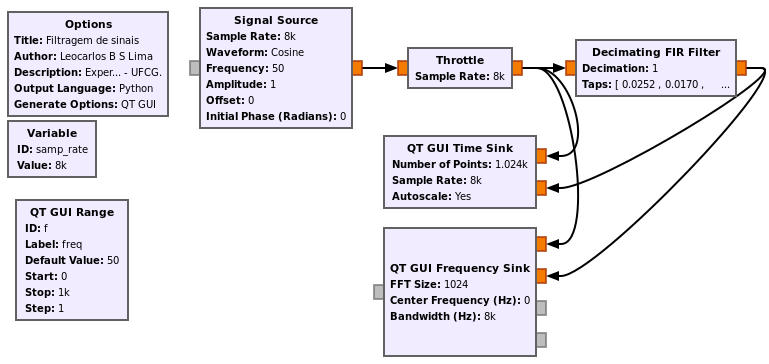
\includegraphics[scale=\myscale]{./Figuras/GRC_2-1a}
        \caption{Diagrama de blocos para análise de filtro passa-baixas projetado em preparação.} 
        \label{fig:GRC_2-1}
    \end{figure}
    % \item Ajuste os parâmetros do bloco \textbf{Noise Source} da seguinte forma:
    % \begin{itemize}
    %     \item \textbf{Noise Type}: Gaussian;
    %     \item \textbf{Amplitude}: 1;
    % \end{itemize}
    \item Preencha o campo \textbf{Taps} do bloco \textbf{Decimating FIR Filter} (filtro FIR) com os pesos $b_i$ calculados na preparação (lista entre colchetes, com taps separados por vírgulas), use $N=25$ pesos;
    \item Execute o diagrama e responda às questões propostas na Folha de Respostas.
\end{enumerate}

\subsection{Experimento 2 -- Relação sinal-ruído de sinal periódico}

O objetivo deste experimento é observar o efeito da relação sinal-ruído sobre um sinal pela inspeção do mesmo nos domínios do tempo e da frequência.

\begin{enumerate}
    \item Abra o arquivo \textbf{Labo2-2.grc} disponibilizado pelo professor. A Figura \ref{fig:GRC_2-2a} ilustra o diagrama deste experimento. Ele consiste numa fonte senoidal adicionada a um ruído gaussiano e de um filtro passa-baixas. Os sinais no tempo, bem como na frequência, são mostrados antes e depois do filtro;
    \begin{figure}[htb]
        \centering
        \includegraphics[width=1.0\linewidth]{./Figuras/GRC_2-2}
        \caption{Diagrama de blocos para análise da relação sinal-ruído.} 
        \label{fig:GRC_2-2a}
    \end{figure}
    \item Ajuste os parâmetros do bloco \textbf{Noise Source} da seguinte forma:
    \begin{itemize}
        \item \textbf{Noise Type}: Gaussian;
        \item \textbf{Amplitude($\sigma$)}: 0.1;
    \end{itemize}
    \item Ajuste os parâmetros do bloco \textbf{Signal Source} da seguinte forma:
    \begin{itemize}
        \item \textbf{Frequency}: 125 Hz;
        \item \textbf{Waveform}: Cosine;
        \item \textbf{Amplitude}: 1;
        \item \textbf{Offset}: 0;
    \end{itemize}
    \item Defina a banda de passagem do bloco \textbf{Low Pass Filter} ajustando a variável \textbf{freqDeCorte} para 2000 Hz;
    \item A potência da senoide (\textbf{Signal Source}), entendida como se esta fosse aplicada a um resistor de $1~\Omega$, é dada por $A^2/2$~W e a potência média do ruído é dada de acordo com o exposto na seção \ref{sec:theorySNR}. Aqui, a variância do ruído é dada por sua amplitude (desvio padrão) ao quadrado $\sigma^2$;
    \item Execute o diagrama e responda às questões propostas na Folha de Respostas.
\end{enumerate}

\subsection{Experimento 3 -- Relação sinal-ruído e largura de faixa de sinal de áudio}

O objetivo deste experimento é observar o efeito da relação sinal-ruído e da largura de faixa de um sinal de áudio subjetivamente, pela audição do áudio, e por inspeção do sinal no domínio da frequência.

\begin{enumerate}
    \item Abra o arquivo \textbf{Labo2-3.grc} disponibilizado pelo professor. A Figura \ref{fig:GRC_2-2b} ilustra o diagrama deste experimento. Ele consiste numa fonte de áudio gravado em arquivo em formato \textit{wave} disponibilizado pelo professor, de uma fonte de ruído, de amplitude ajustável por uma régua deslizante, e de um filtro passa-baixas com a frequência de corte ajustada por uma régua deslizante. Este áudio, após adição do ruído e filtragem por um filtro passa-baixas, é reproduzido nos alto-falantes do computador;
    \item Verifique se o parâmetro \textbf{File} do bloco \textbf{Wave File Source} está com o caminho corretamente direcionado ao arquivo. Corrija se necessário;
    \item Execute o diagrama e responda às questões propostas na Folha de Respostas.
\end{enumerate}

\begin{figure}[t]
    \centering
    \includegraphics[width=1.0\linewidth]{./Figuras/GRC_2-3.png}
    \caption{Diagrama de blocos para análise da relação sinal-ruído.} 
    \label{fig:GRC_2-2b}
\end{figure}\clearpage\pagenumbering{arabic}

\noindent \includegraphics[height=2cm]{../Figuras/UFCGLogo} \hfill
\begin{minipage}{.66\textwidth} \large \centering \vspace{-1.8cm}
    Universidade Federal de Campina Grande -- UFCG \\
    Unidade Acadêmica de Engenharia Elétrica -- UAEE \\
    Curso de Graduação em Engenharia Elétrica
\end{minipage}
\hfill \includegraphics[height=2cm]{../Figuras/DEELogo} \\[12pt]

\noindent
\begin{tabular*}{\textwidth}{l @{\extracolsep{\fill}} r @{\extracolsep{6pt}} l}
    \textbf{\disciplina} && \\
    Período \periodo && \\
    \textbf{\avaliacao\ -- Folha de Respostas} && \\
    Tema(s): \tema && \\
    Professor(es): \professor && \\[12pt]
    \textbf{Aluno:} \hrulefill & \textbf{Data:} \makebox[3cm]{\hrulefill} & \\
\end{tabular*}
\noindent\rule[2ex]{\textwidth}{2pt}

\subsection*{Experimento 1 -- Filtragem de sinais}

\begin{questions}
    \question Observe os gráficos no domínio do tempo, existe um atraso entre os sinais de entrada e de saída (após o filtro). De quanto é esse atraso? Por que esse valor do atraso?
    \fillwithlines{0.5in}
    
    \question Na frequência os sinais são absolutamente iguais, por que?
    \fillwithlines{0.5in}

    \question A frequência de corte do filtro é o ponto onde a potência do sinal de saída do filtro é metade da potência do sinal de entrada, chamado de ponto de 3 dB. A potência do sinal de entrada é $(A^2/2) = 1/2$ W, então a amplitude para qual a potência de saída seja 1/4 W é $A = 1/\sqrt{2} \approx 0,7071$ V. Aumente a frequência da senóide de  modo que a senóide de saída tenha essa amplitude. Qual a frequência em que isso ocorre? Verifique se a diferença é realmete 3 dB no gráfico da frequência. Observe que no projeto estabelecemos uma freuência de corte de 800 Hz.
    \fillwithlines{0.5in}
    
    \question Coloque a frequência da senóide em 1 kHz. O sinal de saída praticamente desapareceu. De quanto, em dB, o sinal de entrada foi atenuado?
    \fillwithlines{0.5in}

    \question Substitua o sinal de entrada por uma onda quadrada, \textbf{Waveform} para Square. A onda quadrada ficou distorcida depois do filtro. Quando aumentamos a frequência essa distorção aumenta, por que?
    \fillwithlines{0.5in}
    
    % \question Ajuste a frequência da onda quadrada para 500~Hz, execute o experimento e explique o que você observou, tanto no tempo como na frequência.
    % \fillwithlines{0.5in}
    
    \question Se quiséssemos gerar uma senoide e tivermos na bancada um gerador de onda quadrada e um filtro passabaixas com características semelhantes a desse experimento, como você faria? Qual seria a frequência mínima da senoide, teórica e na prática?
    \fillwithlines{0.5in}

    \question Substitua o bloco \textbf{Decimating FIR Filter} pelo bloco \textbf{High Pass Filter}, ajuste o parâmetro \textbf{Cutoff Freq} para 400 Hz e o parâmetro \textbf{Transition Width} para 50. Execute o experimento e explique o que você observou.
    \fillwithlines{0.5in}
    
    \question Ajuste a frequência da onda quadrada para uma frequência acima da frequência de corte do filtro passa altas, execute o experimento e explique o que você observou.
    \fillwithlines{0.5in}
    
    \question Substitua o bloco \textbf{Signal Source} pelo bloco \textbf{Noise Source}. Ajuste \textbf{Noise Type}: Gaussian e \textbf{Amplitude}: 1. Execute o experimento. Observe na frequência o formato do filtro passa-altas, esse é um modo prático de examinarmos a característica de um filtro desconhecido, colocamos uma fonte de ruído na entrada e observamos o comportamento na frequência da saída do filtro. No tempo o sinal de saída perdeu potência em relação ao sinal de entrada. Estime em quanto o ruído é atenuado (em dB) na faixa de rejeição do filtro (por exemplo, na frequência de 200 Hz).
    \fillwithlines{0.5in}
\end{questions}

\subsection*{Experimento 2 -- Relação sinal-ruído de sinal periódico}

\begin{questions}
    \question Qual a relação sinal-ruído (SNR) do experimento antes do filtro? E depois do filtro? Observando os gráficos no domínio da frequência, dada a quantidade de componentes de frequência do ruído que são eliminadas pelo filtro, quanto você estima, em dB, o aumento da SNR na saída do filtro? Este valor estimado está de acordo com os valores de SNR mostrados na simulação? (Dica: Eq.~(\ref{eq:SNRdB}))
    \fillwithlines{0.75in}
    
    \question Altere a amplitude da senoide para 2, observe que o sinal melhorou. Em quanto você estima a variação da SNR, em dB, devido a esse aumento de amplitude? Qual a nova SNR do experimento antes do filtro? E depois do filtro?
    \fillwithlines{0.5in}
    
    \question Esse não é o modo mais adequado para se melhorar a relação sinal-ruído, pois aumentar a potência do sinal implica o uso de amplificadores mais caros. Existem maneiras de melhorar a relação sinal-ruído sem aumentar a amplitude do sinal. Sugira uma delas? Implemente a sua sugestão com a amplitude da senoide igual a 1 e execute o experimento para verificar o resultado.
    \fillwithlines{0.5in}
\end{questions}

\subsection*{Experimento 3 -- Relação sinal-ruído e largura de faixa de sinal de áudio}

\begin{questions}
    \question Ajuste a amplitude do ruído, de modo a identificar, em sua opinião, uma degradação máxima aceitável do sinal pelo ruído. Qual a amplitude correspondente? Justifique sua escolha.
    \fillwithlines{1.0in}
    
    \question Observe que a SNR do sinal de áudio (antes e depois do filtro) varia bastante em função do tempo, ao contrário da SNR praticamente constante do sinal senoidal no Experimento~2. Explique as razões desse comportamento.
    \fillwithlines{1.0in}
    
    \question Retire o ruído (reduza amplitude a zero) e ajuste a frequência de corte do filtro passa-baixas de modo a identificar a frequência de corte a partir da qual perde-se a capacidade de identificar o locutor e a frequência de corte a partir da qual perde-se a inteligibilidade do que é dito no áudio. Quais são?
    \fillwithlines{0.5in}
\end{questions}

\end{document}
